\documentclass[./main.tex]{subfiles}

\begin{document}
\section{Preprocessamento ed analisi esplorativa}
Ciascun segnale è stato suddiviso in intervalli di ampiezza \SI{1.5}{s}, che sono stati utilizzati come unità statistiche. Dal momento che ciascuna unità è una serie storica, è stato necessario riassumerle con delle variabili:
\begin{table}[H]
	\centering
	\begin{tabular}{ll}
		\texttt{minA}& Minimo dell'accelerazione.\\
		\texttt{medA}& Mediana dell'accelerazione.\\
		\texttt{varA}& Varianza dell'accelerazione.\\
		\texttt{maxA}& Massimo dell'accelerazione.\\
		\texttt{meanA}& Media dell'accelerazione.\\
		\texttt{MVDeriv}& Media del valore assoluto della derivata seconda.
	\end{tabular}
\end{table}
Siccome i segnali di {\em shake} sono ad alta frequenza, è stata utilizzata la variabile \texttt{MVDeriv} per discriminare le alte frequenze dalle basse frequenze. Infatti, \texttt{MVDeriv} assume valori grandi quando la curvatura della funzione è mediamente elevata nell'intervallo, cioé quando la frequenza è alta. La derivata nell'intervallo è stata approssimata con\cite{NumpyGradientNumPy}
\[
\hat{f}'(t_i) = \dfrac{f(t_i + \Delta t) - f(t_i - \Delta t)}{2\Delta t} + \mathcal{O}(\Delta t^2)\,.
\]

Come prima analisi esplorativa, sono state valutate le distribuzioni delle variabili riassuntive per le varie classi (Figura~\ref{fig:marginali}). \textbf{Scrivere differenze\dots}
%\begin{figure}[H]
%	\centering
%	\includegraphics[width=.8\textwidth]{mettere/grafici/delle/esplicative}
%	\caption{{ t-SNE per i dati sbiancati}}
%	\label{fig:marginali}
%\end{figure}

Per valutare graficamente la separabilità delle classi, l'informazione migliore è data dal t-SNE sui dati sbiancati (Figura~\ref{fig:tsne}). Le componenti principali, invece, non riescono a separare le classi in modo soddisfacente (Appendice A).
\begin{figure}[H]
	\centering
	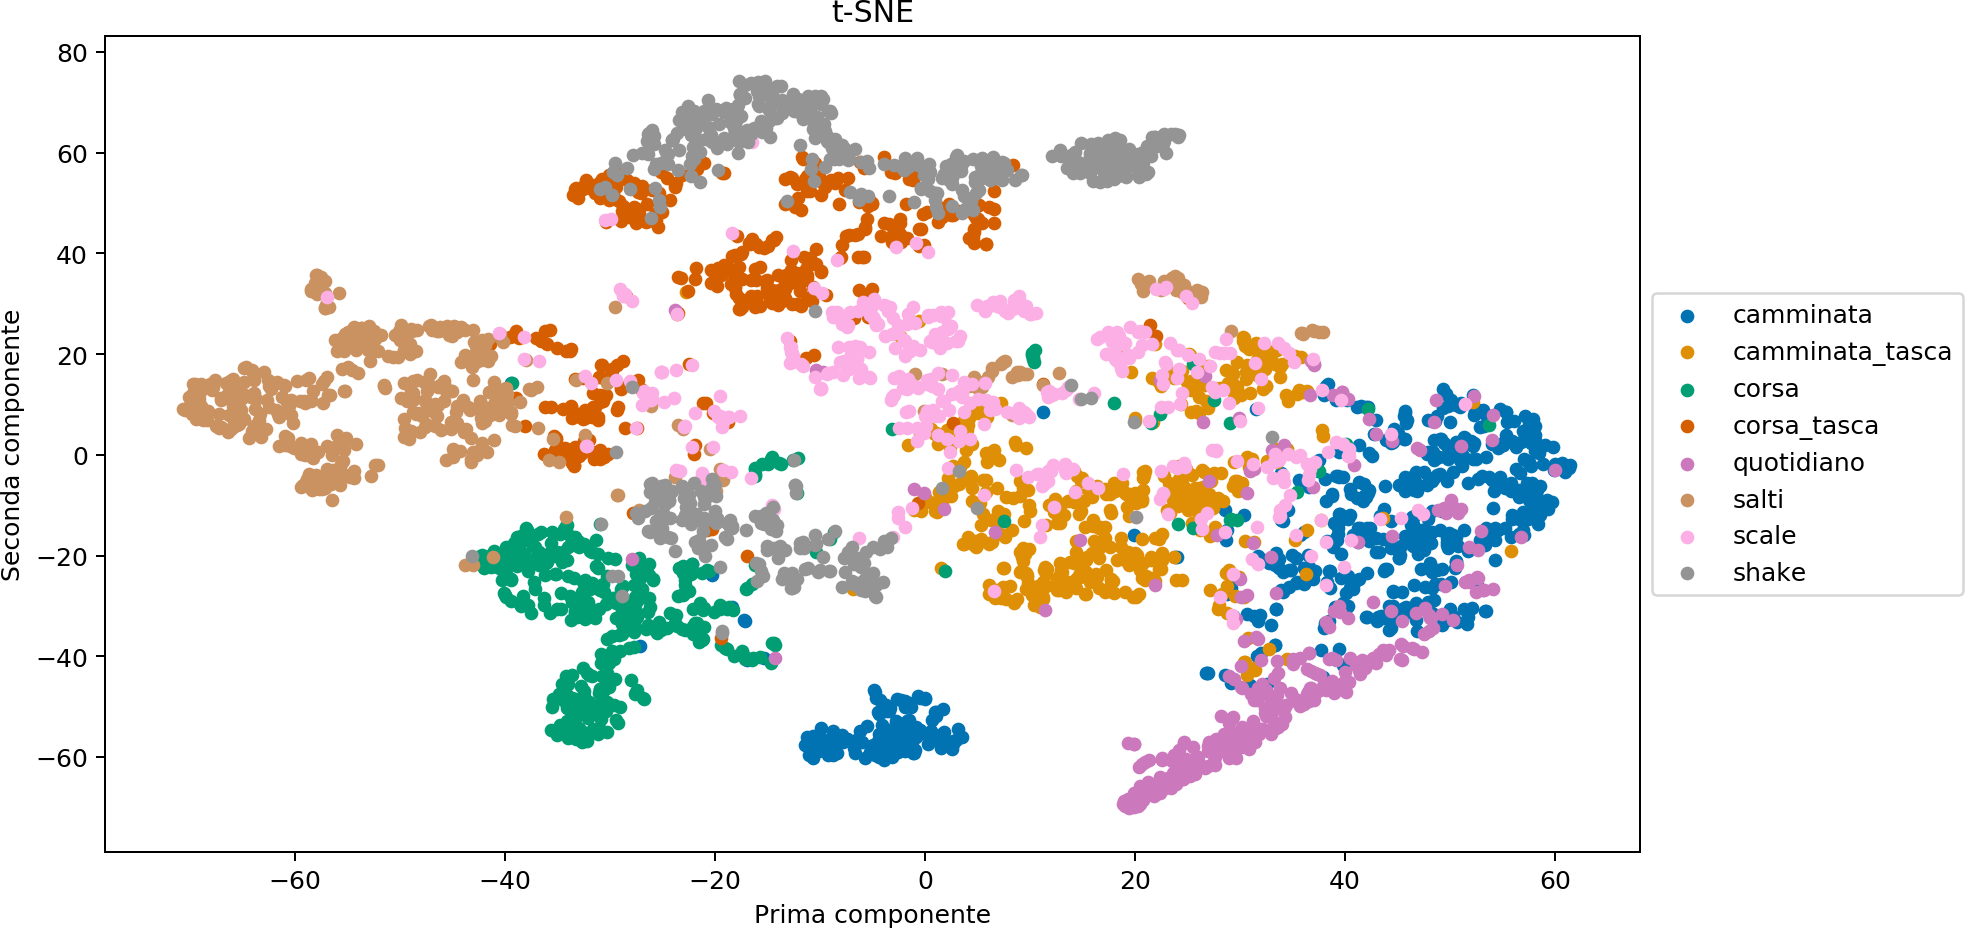
\includegraphics[width=.8\textwidth]{../../figure/t-SNE.png}
	\caption{{ t-SNE per i dati sbiancati}}
	\label{fig:tsne}
\end{figure}
\end{document}